%%%author wuyou
\documentclass[compress,mathserif,serif]{ctexbeamer}
%%一个适合博士/硕士开题或者答辩使用的beamer模板

\definecolor{nudtgreen1}{RGB}{25,83,51}
\definecolor{nudtgreen2}{RGB}{33,77,72}
\definecolor{nudtgreen3}{RGB}{31,52,31}
\mode<presentation>
{
  \useoutertheme[footline=authorinstitute]{wuyoutree}
  \setbeamercolor*{palette primary}{use=structure,fg=white,bg=nudtgreen1}
  \setbeamercolor*{palette secondary}{use=structure,fg=white,bg=nudtgreen1}
  \setbeamercolor*{palette tertiary}{use=structure,fg=white,bg=nudtgreen3}
  \setbeamercolor*{palette quaternary}{fg=white,bg=nudtgreen3}

  \setbeamercolor*{sidebar}{use=structure,bg=structure.fg}
  \setbeamercolor*{palette sidebar primary}{use=structure,fg=structure.fg!10}
  \setbeamercolor*{palette sidebar secondary}{fg=white}
  \setbeamercolor*{palette sidebar tertiary}{use=structure,fg=structure.fg!50}
  \setbeamercolor*{palette sidebar quaternary}{fg=white}

  \setbeamercolor*{titlelike}{parent=palette primary}

  \setbeamercolor*{separation line}{}
  \setbeamercolor*{fine separation line}{}

\setbeamercolor*{section in toc}{fg=black}
\setbeamercolor*{section number projected}{bg=nudtgreen1, fg=white}
\setbeamercolor*{subsection number projected}{bg=nudtgreen1, fg=white}

\setbeamertemplate{items}[circle]
\setbeamercolor*{enumerate subitem}{fg=nudtgreen1}
\setbeamercolor*{itemize item}{bg=nudtgreen1, fg=white}
\setbeamercolor*{itemize item}{fg=red} 

  \useinnertheme{rounded}

  \usefonttheme[onlylarge]{structuresmallcapsserif}
  \usefonttheme[onlysmall]{structurebold}
  %\usecolortheme{seagull}%白底,黑色,适合投影仪效果不好的时候
  %\setbeamercovered{transparent}
  % or whatever (possibly just delete it)
}
\setbeamercolor{background}{bg=yellow!20}
\newcommand{\emptypar}{\par~\par} %一个空行
\newcommand{\yihao}{\fontsize{26bp}{32.5bp}\selectfont}    % 一号, 1.25倍行距
\newcommand{\xiaoyi}{\fontsize{24bp}{30bp}\selectfont}    % 小一, 1.25倍行距
\newcommand{\erhao}{\fontsize{22bp}{27.5bp}\selectfont}    % 二号, 1.25倍行距
\newcommand{\xiaoer}{\fontsize{18bp}{18bp}\selectfont}    % 小二, 单倍行距
\newcommand{\sanhao}{\fontsize{16bp}{24bp}\selectfont}    % 三号, 1.5倍行距
\newcommand{\xiaosan}{\fontsize{15bp}{22.5bp}\selectfont}    % 小三, 1.5倍行距
\newcommand{\sihao}{\fontsize{14bp}{21bp}\selectfont}    % 四号, 1.5倍行距
\newcommand{\banxiaosi}{\fontsize{13bp}{19.5bp}\selectfont}    % 半小四, 1.5倍行距
\newcommand{\xiaosi}{\fontsize{12bp}{18bp}\selectfont}    % 小四, 1.5倍行距
\newcommand{\dawu}{\fontsize{11bp}{11bp}\selectfont}    % 大五号, 单倍行距
\newcommand{\wuhao}{\fontsize{10.5bp}{10.5bp}\selectfont}    % 五号, 单倍行距
\newcommand{\xiaowu}{\fontsize{9bp}{9bp}\selectfont}      %小五,单倍行距
\newcommand{\liuhao}{\fontsize{7.5bp}{7.5bp}\selectfont} %六号,单倍行距
\newcommand{\xiaoliu}{\fontsize{6.5bp}{6.5bp}\selectfont} %小六,单倍行距
\newcommand{\qihao}{\fontsize{5.5bp}{5.5bp}\selectfont}  %七号,单倍行距

\newcommand{\song}{\CJKfamily{song}}    % 宋体   (Windows自带simsun.ttf)
\newcommand{\fs}{\CJKfamily{fs}}        % 仿宋体 (Windows自带simfs.ttf)
\newcommand{\kai}{\CJKfamily{kai}}      % 楷体   (Windows自带simkai.ttf)
\newcommand{\hei}{\heiti}      % 黑体   (Windows自带simhei.ttf)
\newcommand{\xihei}{\CJKfamily{xihei}}      % 黑体   (Windows自带)
\newcommand{\li}{\CJKfamily{li}}        % 隶书   (Windows自带simli.ttf)
\newcommand{\you}{\CJKfamily{you}}      % 幼圆   (Windows自带simyou.ttf)
 
\setbeamertemplate{frametitle}
{  \textbf{\color{black}\insertframetitle}\\[-5pt]
  {\color{blue}\dotfill}
}

\usepackage[english]{babel}
% or whatever 
 
% or whatever
\usepackage{alltt}
\usepackage{amsmath}
\usepackage{amssymb}
\usepackage{amsmath,amssymb,amsfonts}
\usepackage{newtxtext}
\usepackage{multimedia}
 
\usepackage{verbatim}
\usepackage{fancyvrb}
\usepackage{pgf}
\usepackage{tikz}
\usetikzlibrary{arrows,shapes}
\usepackage{graphicx}
\usepackage{subfigure}
\usepackage{xmpmulti}
% \usepackage{chicago}
\bibliographystyle{chinesebst}
% \bibliographystyle{ieee}
\usepackage{hyperref}

\graphicspath{{figures/}}

% Or whatever. Note that the encoding and the font should match. If T1
% does not look nice, try deleting the line with the fontenc.


\title[基于xxxxxxx研究] % (optional, use only with long paper titles)
%\title{国防科技大学开题/答辩报告模版 }
{\color{white}\heiti 基于xxxxxxx研究}
\subtitle[硕士开题报告]
{开题答辩报告}

\author[x~x] % (optional, use only with lots of authors)
{
 硕士生:x~x \\\\
  \hspace{2em}导~~~~师:xx研究员\\ \hei
  \quad \\
 % \scriptsize{Email: yangjing2036@126.com}
  }


% - Use the \inst{?} command only if the authors have different
% affiliation.
\institute[国防科技大学] % (optional, but mostly needed)
{
  国防科技大学计算机学院
 % \\国产基础软件工程中心
}

%可以自己定制日期
%\date[2022年03月15日] % (optional)
%{2022年03月15日}

\date[] % (optional)
{\today}

\subject{Talks}
% This is only inserted into the PDF information catalog. Can be left
% out.

\pgfdeclareimage[height=1cm]{logo}{nudt_logo}
\logo{\pgfuseimage{logo}}



% \AtBeginSection[] {
%   \begin{frame}<beamer>
%     \kai
%     \frametitle{提纲}
%     \tableofcontents[currentsection,hideallsubsections]
%     \hei
%   \end{frame}
% }
\AtBeginSubsection[] {
  \begin{frame}<beamer>
    \frametitle{提纲}
    {\xiaowu \tableofcontents[currentsection,currentsubsection]}
    \hei
  \end{frame}
}


% If you wish to uncover everything in a step-wise fashion, uncomment
% the following command:

% \beamerdefaultoverlayspecification{<+->}


\begin{document} 
  \begin{frame}
    \titlepage
  \end{frame}

  % \begin{frame}
  %   \frametitle{提纲}
  %   \tableofcontents
  %   %   You might wish to add the option [pausesections]
  % \end{frame}
  \begin{frame}
    \frametitle{目录}
    {  \xiaowu
      \tableofcontents[hideallsubsections]
      \heiti}
  \end{frame}


  \newcommand{\tspr}{~$TSPR$~}

%%%%%%%%%%%%%%%%
\section{课题背景及意义}
\label{Introduction:background}
%%%%%%%%%%%%%%%%%%%%%%%%%%%%%%%%%%%%%%%%%%%%%%%%%%%%%

\subsection{课题背景}
\label{sec:back}

\frame{
\frametitle{太极拳背景介绍}
\begin{itemize}
\item 太极拳好~\cite{taiji}~
\item 太极拳非常好
\end{itemize}
{\alert{本课题来源于于国家~863~项目:太极拳和三个代表(No. 123456789)}}


}

%%%%%%%%%%%%%%%%%%%%%%%%%%%%%%%%%%%%%%%%%%%%%%%%%%%%%
\frame{
\frametitle{太极拳无敌}
\begin{center}
 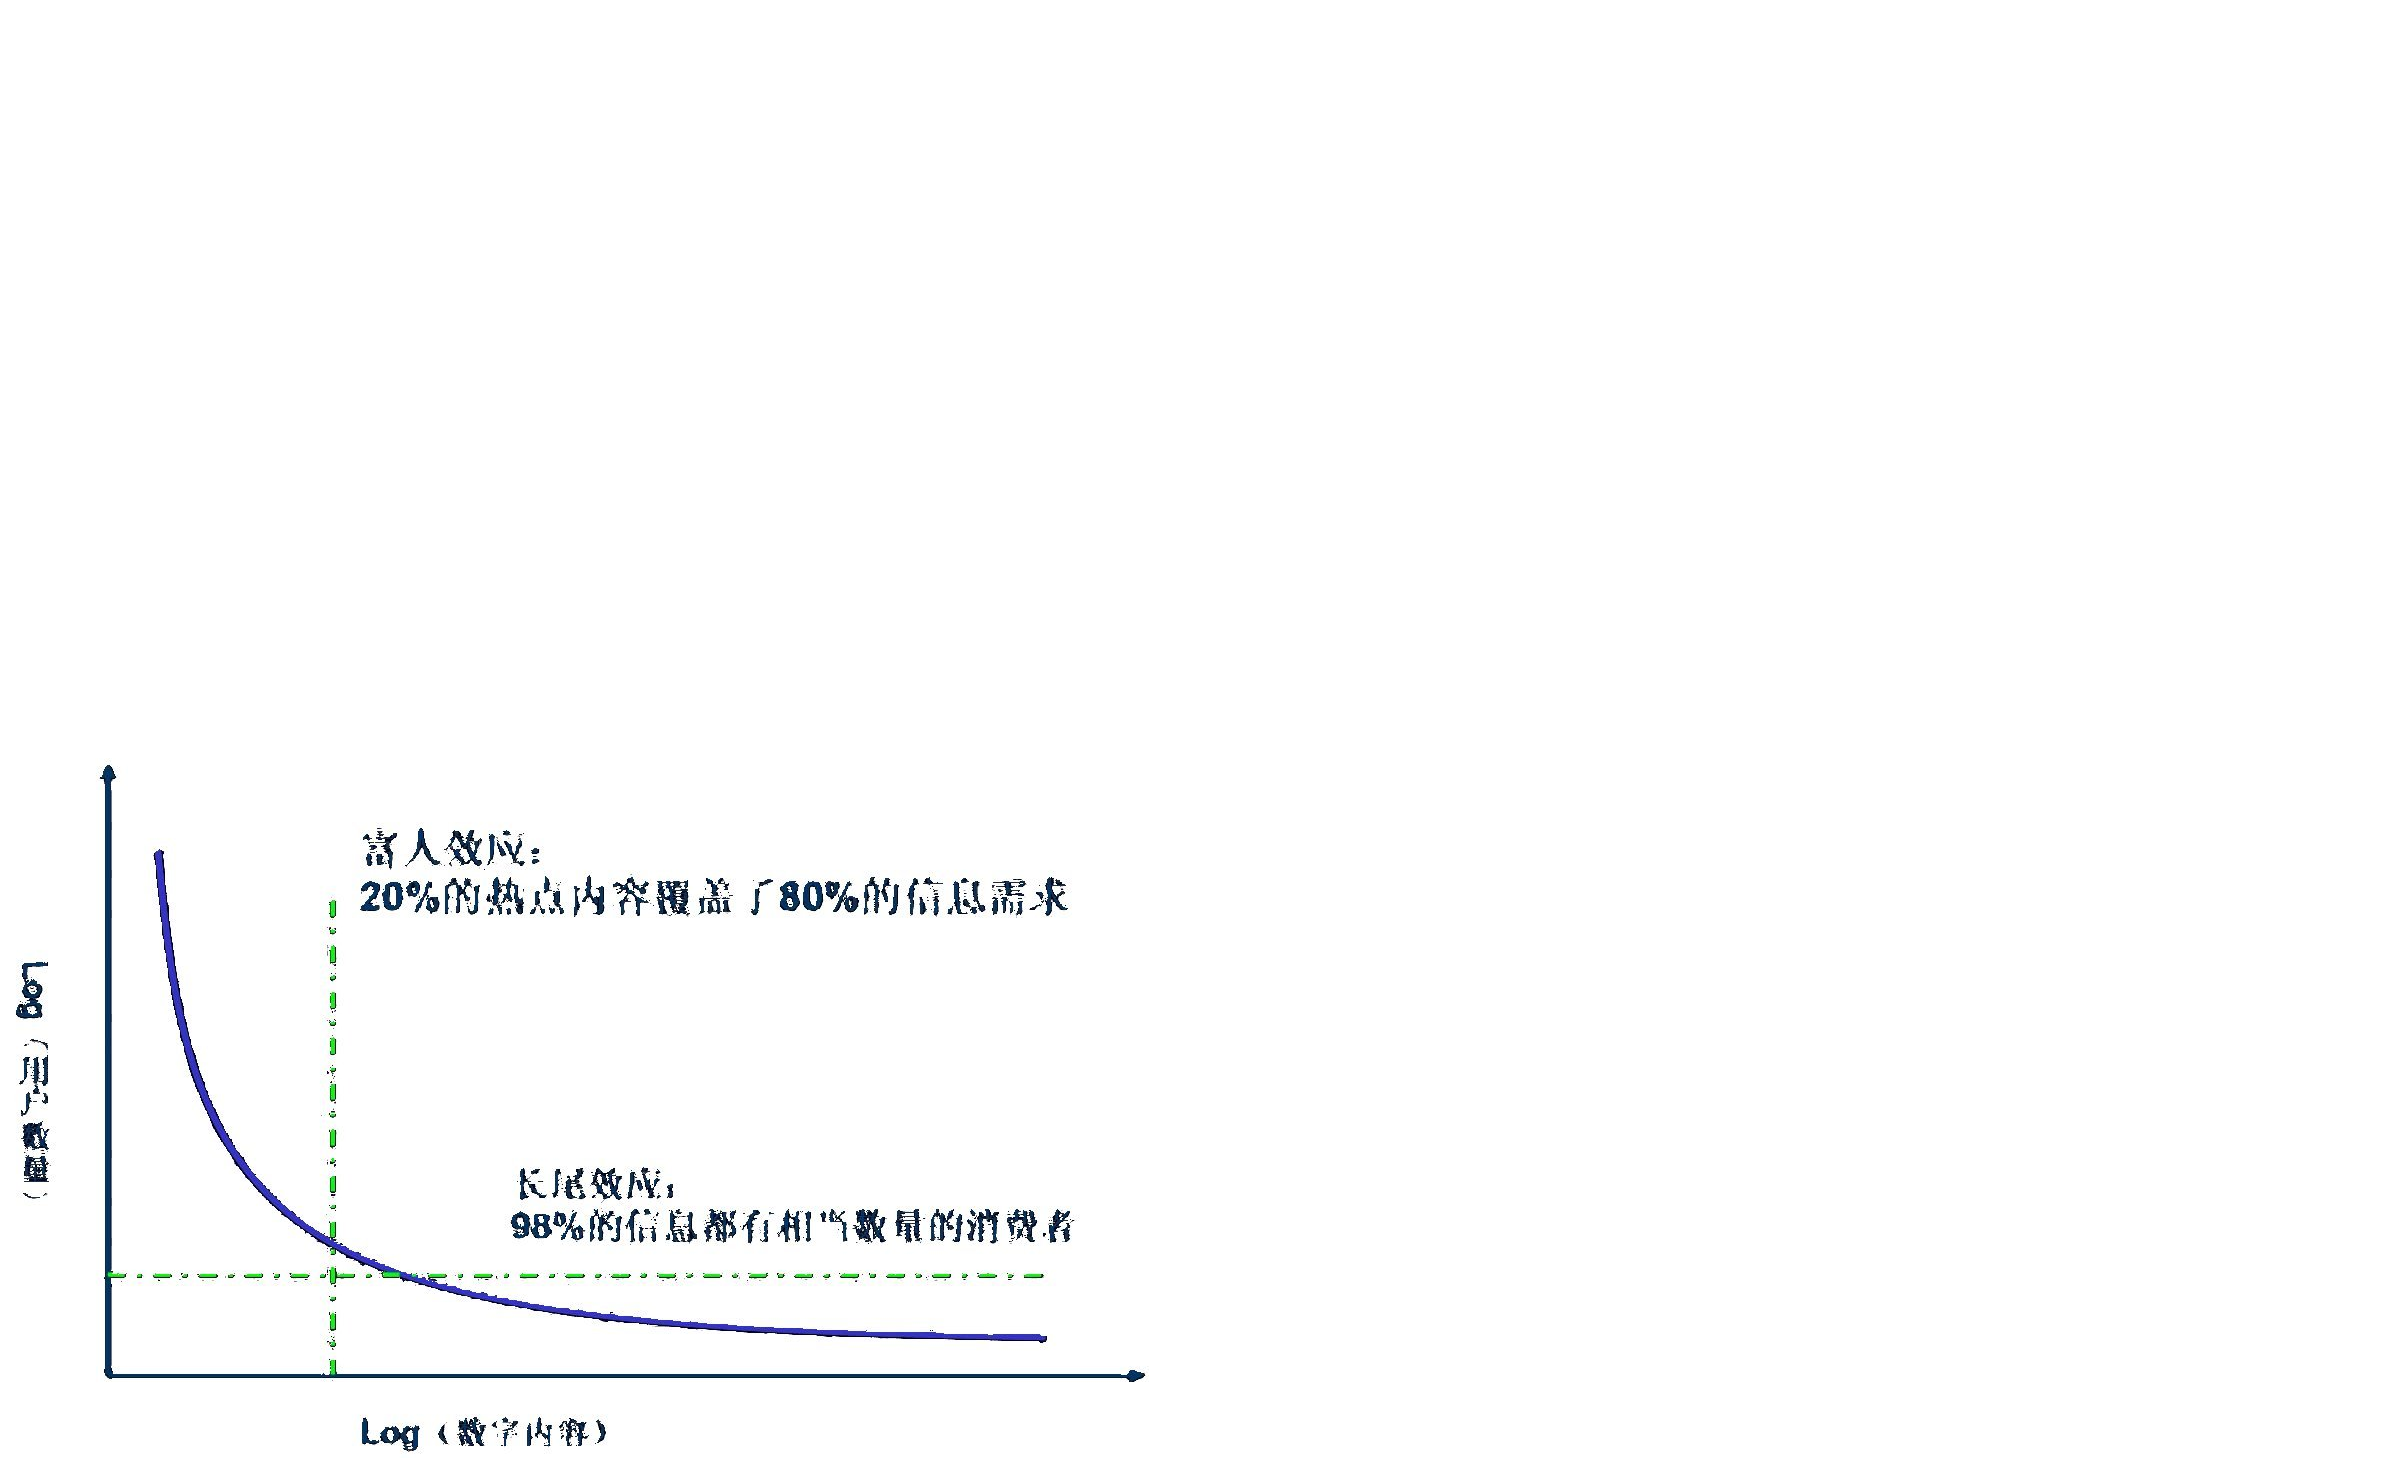
\includegraphics[height=2.5cm]{long-tail.pdf}
\end{center}
\begin{itemize}
\item 太极包容一切
\item 太极代表一切
\end{itemize}
}

%%%%%%%%%%%%%%%%%%%%%%%%%%%%%%%%%%%%%%%%%%%%%%%%%%%%%

\subsection{研究意义}
\label{sec:means}

\frame{
\frametitle{研究的意义}
\begin{itemize}
\item 意义
\end{itemize}
}

%%%%%%%%%%%%%%%%%%%%%%%%%%%%%%%%%%%%%%%%%%%%%%%%%%%%%
\section{国内外研究现状分析}
\label{sec:researchsituation}
%%%%%%%%%%%%%%%%%%%%%%%%%%%%%%%%%%%%%%%%%%%%%%%%%%%%%
\frame{
\frametitle{太极独步天下}

\begin{itemize}
\item 无人能敌
\item 暂不外传
\end{itemize}
}

\section{主要研究内容和方案}
\label{sec:researchplan}
%%%%%%%%%%%%%%%%%%%%%%%%%%%%%%%%%%%%%%%%%%%%%%%%%%%%%
\frame{
\frametitle{总体研究思路}
}
 

\subsection{太极剑}
\label{sec:topic_crawler}
%%%%%%%%%%%%%%%%%%%%%%%%%%%%%%%%%%%%%%%%%%%%%%%%%%%%%
 
%%%%%%%%%%%%%%%%%%%%%%%%%%%%%%%%%%%%%%%%%%%%%%%%%%%%%
\frame{
\frametitle{太极剑研究内容}
见于相关论文的方法主要有以下几种:
\begin{itemize}
\item 基于“内功”的方法
\item 基于“招式”方法。
\item 其他方法
\end{itemize}

}
%%%%%%%%%%%%%%%%%%%%%%%%%%%%%%%%%%%%%%%%%%%%%%%%%%%%%
\frame[allowframebreaks]{
\frametitle{常用链接分析方法}
最为有效的两种传统方法是PageRank~\cite{pagerank}~和HITS~\cite{hits}~。

PageRank方法是~L. Page~和~S. Brin~于1998年提出的基于网络链接分析对网页
排序的方法。最初是用来对搜索引擎返回的结果页面进行排序,以完成网页的自
动排名和提高搜索引擎的服务质量。
一些相关定义:
\begin{definition}{$I(v)$~:}
  网页~$v$~的入度。即,指向网页~$v$~的网页数目
\end{definition}
\begin{definition}{$O(v)$~:}
网页~$v$~的出度,即网页指向~$v$~的网页数目
\end{definition}
\begin{definition}{$N$~ :}
网页集合~$W$~的网页数量
\end{definition}
\begin{definition}{ $d$~ :}
在随机浏览模型中,用户从一个网页随机跳到另外一个网页的概率
\end{definition}
\begin{definition}{$p\rightarrow q$ :}
存在从网页~$p$~到网页 ~$q$~的一个超链接
\end{definition}
令~$PR(i)$~表示网页~$i$~的排序值,则最基本的PageRank~方法可以形式化描述如下:
\begin{equation}
  \label{eq:page-rank}
  PR(i)=(1-d) \sum_{j:j \rightarrow i}{\frac{ PR(j)}{O(j)} }+d\frac{1}{N}
\end{equation}

}
%%%%%%%%%%%%%%%%%%%%%%%%%%%%%%%%%%%%%%%%%%%%%%%%%%%%%


\subsection{太极脚}
\label{sec:web_social}
%%%%%%%%%%%%%%%%%%%%%%%%%%%%%%%%%%%%%%%%%%%%%%%%%%%%%

\section{前期研究与试验工作}
\label{sec:prework}


\subsection{太极起步阶段}
\label{sec:step}
%%%%%%%%%%%%%%%%%%%%%%%%%%%%%%%%%%%%%%%%%%%%%%%%%%%%%
\frame{
\frametitle{太极起步}
\begin{figure}[htbp]
\centering
  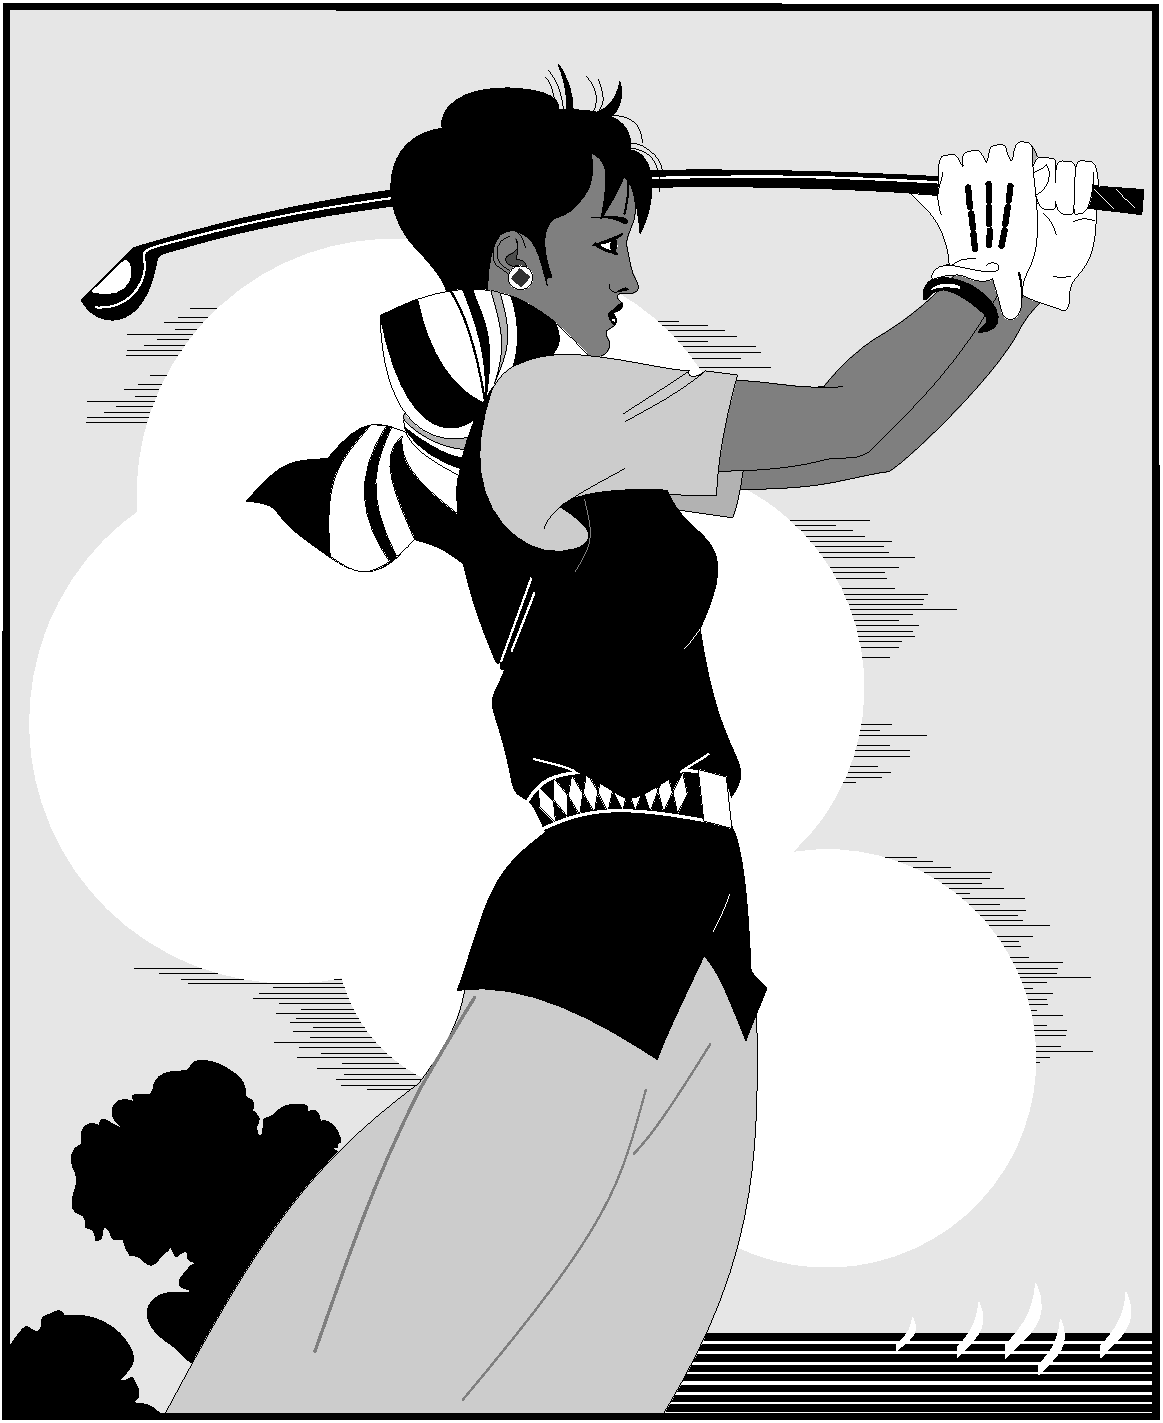
\includegraphics[width = 3cm]{golfer.pdf}
\label{Figure:research}
\end{figure}

}
%%%%%%%%%%%%%%%%%%%%%%%%%%%%%%%%%%%%%%%%%%%%%%%%%%%%%



\section{论文进度安排和预期目标}
\label{sec:destination}
%%%%%%%%%%%%%%%%%%%%%%%%%%%%%%%%%%%%%%%%%%%%%%%%%%%%%
\frame{
\frametitle{已经完成的工作}
\begin{itemize}
\item 太极1
\item 太极2
\end{itemize}
}
%%%%%%%%%%%%%%%%%%%%%%%%%%%%%%%%%%%%%%%%%%%%%%%%%%%%%
\frame[allowframebreaks]{
\frametitle{时间安排}
拟定工作时间从xxxx年x月至明xxxx年xx月,初步安排如下:
\begin{itemize}
\item xx年x月-x月:进一步完善太极拳
\item xx年x月-x月:进一步完善太极剑
\item xx年x月-x月:进一步完善太极脚
\item xx年x月:开始撰写毕业论文
\end{itemize}

}

%%%%%%%%%%%%%%%%%%%%%%%%%%%%%%%%%%%%%%%%%%%%%%%%%%%%%
\frame{
\frametitle{预计发表论文}
预计毕业时间:xx年xx月-xx年底
预计发表论文:x-y篇
}

\section{完成课题已具备和所需条件及经费}
\label{sec:require}
%%%%%%%%%%%%%%%%%%%%%%%%%%%%%%%%%%%%%%%%%%%%%%%%%%%%%
\frame{
\frametitle{完成课题已具备和所需条件及经费}
进行工作的必要条件已经全部具备
\begin{itemize}
\item 本研究依托于国家~863~项目:
\item 研究室可以提供计算机、上机时间、相关软件、上网查找资
料等条件,以及提供与课题有关的一些书籍供阅读学习
\item 学校的图书馆可以提供阅览书籍和相关文献的条件。
\end{itemize}
}


\section{研究中可能遇到的困难、问题,以及解决途径}
\label{sec:problem_resolve}
%%%%%%%%%%%%%%%%%%%%%%%%%%%%%%%%%%%%%%%%%%%%%%%%%%%%%
\frame{
\frametitle{困难、问题,以及解决途径}
\begin{itemize}
\item 问题1:无影脚凶狠
\item 问题2:九阴白骨抓阴毒
\item 问题3:美女关难过
\end{itemize}
}
\begin{center}
{\hei \bf 主要参考文献\\}
\end{center}
\bibliography{reference}
%%%%%%%%%%%%%%%%%%%%%%%%%%%%%%%%%%%%%%%%%%%%%%%%%%%%%

\frame[plain, label=last]{
\vspace{2.5cm}
\hspace{1.7cm}
%\includegraphics{Thanks.pdf}
\xiaoer  \begin{center} \textbf{\textit{Thanks for your attention! \\  \emptypar Q \& A }}\end{center}
\vspace{1.5cm}
\begin{flushleft}
 \small 答辩人:xxx\\[1.5pt]电话:xxxxx  \\[1.5pt] 邮件:xxxxx@126.com \\[1.5pt]  学院:国防科技大学计算机学院\\[1.5pt]
\end{flushleft}
}
 
\end{document}
